

\begin{block}{The Experiment}
%TODO Get rid of 4panel, put the top left picture, include text/caption explaining the setting based on picture added
% TODO State machine from the slides with updated transition probs.
% 0.86 stay in bad
% 0.14 transition to good
\begin{itemize}
    \item In a simulated housing market, participants needed to decide whether to sell or wait in order to gain more information.
    \item Waiting decreases risk, but increases costs.
    \item 24 participants performed three different scenarios.
\end{itemize}

\begin{figure}
  \centering
    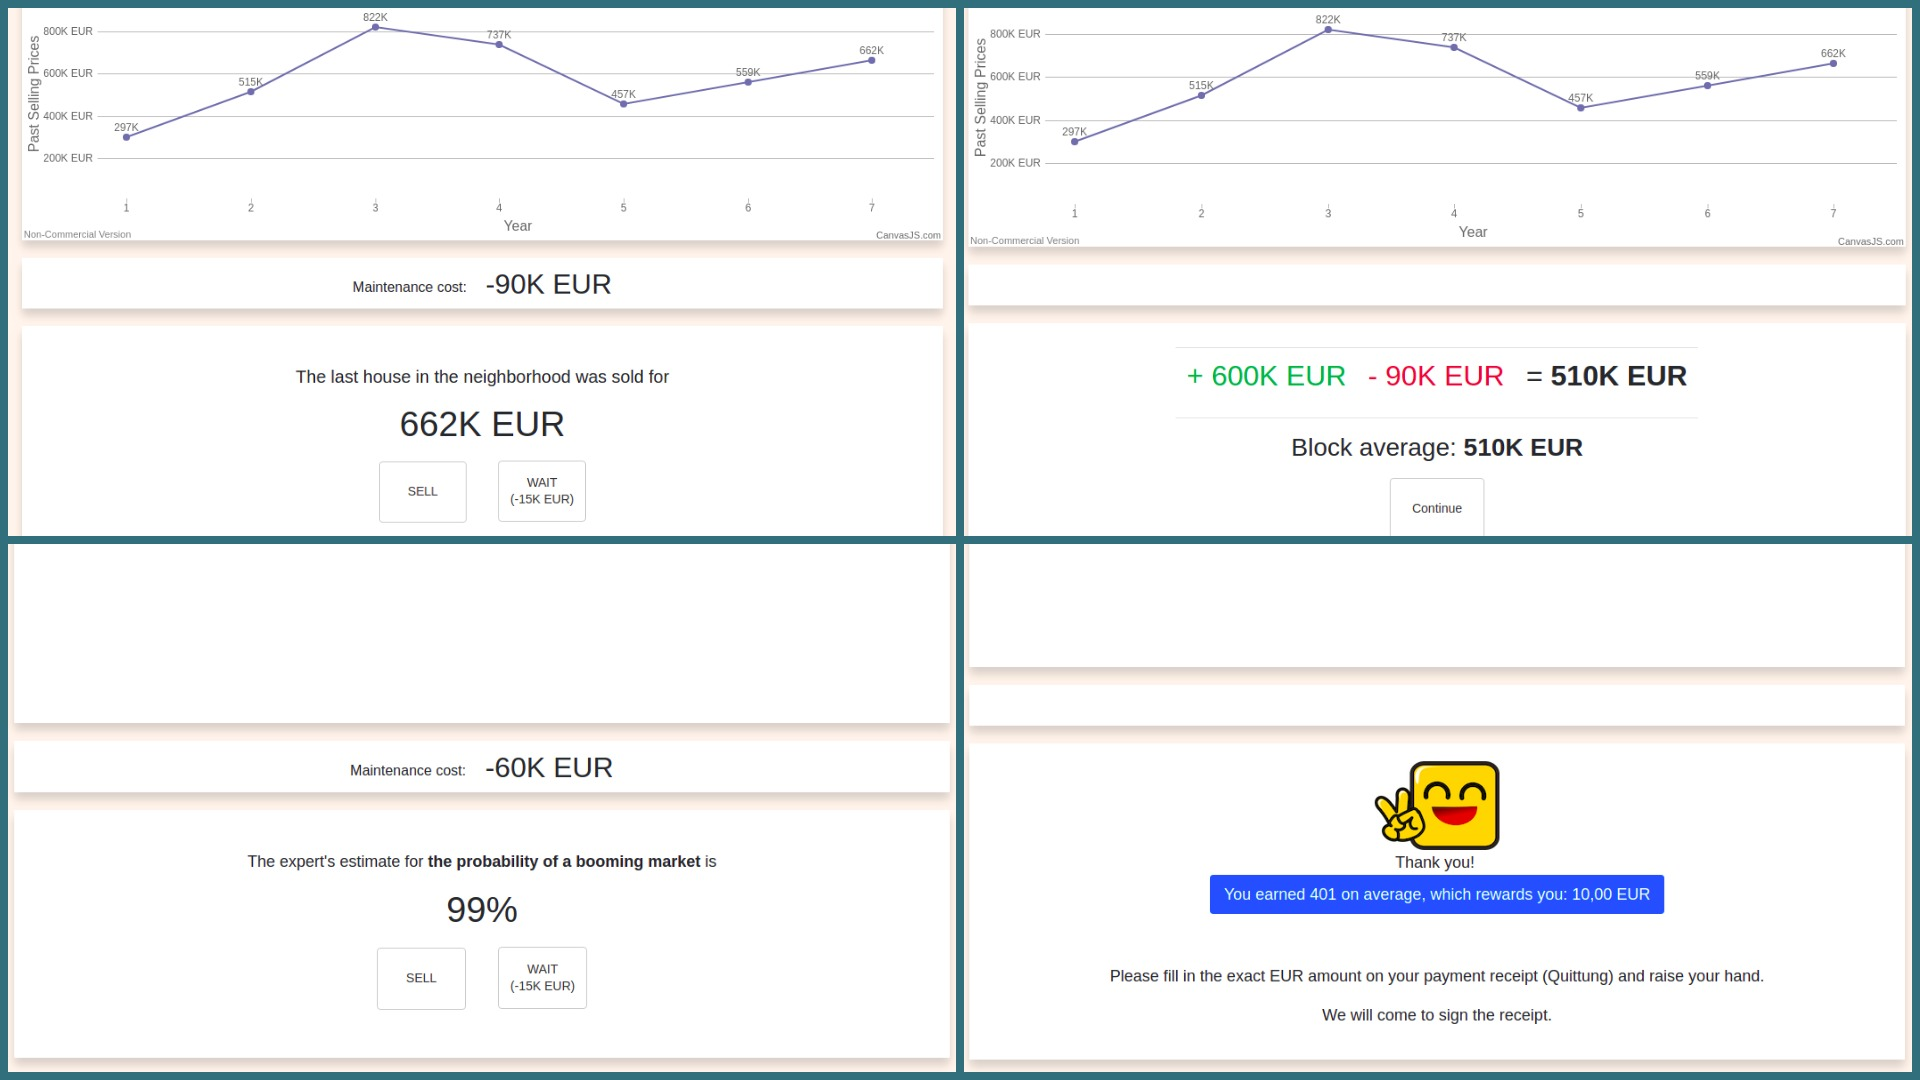
\includegraphics[width=0.9\textwidth]{img/methods/pjimage.jpg}
  \caption{UI showing the observation history.}
\end{figure}

\end{block}


\begin{block}{The Agent}



\begin{itemize}
    \item Simplify POMDP into a MDP by Bayesian estimates. % TODO add belief transition table (point 1)
    \item Solve the MDP with value iteration on an augmented state space.
    % TODO formula for value iteration, expected values separated if it doesn't fit
    \[V^{(n-1)}(b,w) =\ldots\]
    \item Different utility functions.
    % formulas for different utility functions.
\end{itemize}

\end{block}

